%%
%% neuralfields.tex
%% 
%% Made by jjfigueredou
%% Login   <jjfigueredou@fctp-jjfu>
%% 
%% Started on  Sun Oct  5 12:26:22 2008 jjfigueredou
%% Last update Sun Oct  5 12:26:22 2008 jjfigueredou
%%

\documentclass{sig-alternate}

\usepackage{algorithm}
\usepackage{algorithmic}

\begin{document}
%
% --- Author Metadata here --- \conferenceinfo{WOODSTOCK}{'97 El Paso,
%   Texas USA}
% \CopyrightYear{2007} % Allows default copyright year (200X) to be over-ridden - IF NEED BE.
% \crdata{0-12345-67-8/90/01} % Allows default copyright data (0-89791-88-6/97/05) to be over-ridden - IF NEED BE.
% --- End of Author Metadata ---

\title{Evolved Neural Fields Applied to the Stability Problem of a
  Simple Biped Walking Model} \subtitle{[Track: Artificial Life,
  Evolutionary Robotics, Adaptive Behavior, Evolvable Hardware]}

\numberofauthors{2}

% \author{
% %   1st. author
%   \alignauthor
%   Juan Figueredo\\
%   \affaddr{Universidad Nacional de Colombia}\\
%   \affaddr{Ciudad Universitaria}\\
%   \affaddr{Bogot�, Colombia}\\
%   \email{jjfigueredou@unal.edu.co}
% %   2nd. author
%   \alignauthor
%   Jonatan G�mez\\
%   \affaddr{Universidad Nacional de Colombia}\\
%   \affaddr{Ciudad Universitaria}\\
%   \affaddr{Bogot�, Colombia}\\
%   \email{jgomezpe@unal.edu.co} }

\maketitle

\begin{abstract}
  The neural field model has the potential to address goal-based
  planning problems but has not been significantly applied to dynamic
  control problems. We propose a control architecture based on neural
  fields which is suitable to perform the control of a relatively
  complex and unstable system. We propose a strategy for the evolution
  of the kernel function for each population on the field. We test it
  over the stability problem on a typical inverted-pendulum and
  compare the performance of an evolved neural field and a hand-tuned
  neural field. There are presented some relevant requirements for the
  neural field controller architecture and its parameterization by
  evolution, and the controller architecture is detailed. Remarkably,
  the neural field controller performs well in the simulation and has
  a spatial representation which allows interpretation of field
  potentials. Also, the evolved neural field performs better than the
  non-evolved one, but uses a different strategy to control the plant.
\end{abstract}

\category{I.2.8}{Artificial Intelligence}{Problem Solving, Control
  Methods, and Search}[control theory]

\category{I.2.6}{Artificial Intelligence}{Learning}[connectionism and
neural nets]

\category{I.2.9}{Artificial Intelligence}{Robotics}[kinematics and
dynamics]

\terms{Algorithms, Design}

\keywords{Neural fields, neurocontrol, evolutionary robotics,
  artificial life}

\section{Introduction}
Artificial life aims to find those emergent phenomena that give
complex attributes to the existent living beings. In this work,
efforts are directed towards the study of emergence of motion control
capabilities and dynamical planning behaviors of biped walking
agents. Following the artificial life approach
\cite{Nolfi04Evolutionary}, those capabilities are expected to emerge
from a very simple or non-functional initialization, in this case
using a neural control architecture.

In biped robotics, the methods based on computational intelligence for
planning and control have shown to be able to achieve static stability
\cite{Kun97Adaptive}, dynamical stability
\cite{Nakanishi2004b,Komatsu05Dynamic}, achieve simple control
structures \cite{Huelse04Structure}, and tolerate perturbations
\cite{Juang02Intelligent}. Nonetheless, those properties have not been
extended to an integrated architecture of planning and control capable
of following goals.

Here is proposed a control scheme based on neural fields and a
comparison is made between a hand-tuned controller and a controller
parameterized by an evolutionary algorithm. As controller, the neural
fields, compared with recurrent neural networks, have a deeper
biological basis, apply more restrictions and extend the discrete
model to a continuous one, following the method of planning and
control by means of neural fields \cite{Bergener99Complex}. The neural
field model, as noted in the article by Bergener et al., has the
potential to address goal-based planning problems, so we are here
interested on its capability to solve dynamic control problems.

The control problem set for testing the architectures is the stability
problem on an inverted pendulum, so that the controller ability to
perform dynamic control on an unstable plant can be evaluated. To the
authors' knowledge this is the first time neural fields parameterized
by evolutionary algorithms have been evaluated for solving a control
problem for an unstable plant.

First, some preliminaries on computational intelligence are presented,
mainly in the area of neural fields, which is the main focus of the
article, and in the area of evolutionary computation. In the remaining
sections the control problem used as test bed is detailed, the neural
field control architecture is presented and the strategies for its
manual parameterization and parameterization by evolution are shown,
the experimental results are presented, and finally, a discussion is
made.


\section{Preliminaries on Computational Intelligence}
\subsection{Recurrent Neural Networks and Neural Fields}
Artificial neural networks are a connectionist computing scheme
inspired by brain neural layout at cellular level. It is based on
simple computing structures called neurons which have several inputs
and a single output.

Recurrent neural networks present a dynamic behavior because of its
memory, that is, each state depends of the previous state in such a
way that a difference equation arises. There is not a notion of
locality in this model and the interactions between neurons and inputs
is given by parameter matrices.

Neural fields, on the other hand, arise as a tissue level model of
neural populations in brain. The model has been proposed by Wilson and
Cowan \cite{Wilson72Excitatory} and detailed by Amari
\cite{Amari77Dynamics} in the particular case of lateral
inhibition. In this model, neural population in considered a continuum
in which exists a dynamical evolution equation where the mean
activation potential evaluated in one place is affected by its
neighborhood, according to a so-called mexican hat function (as noted
by Coombes \cite{Coombes05Waves} better called wizard hat function),
in which close neighbors act as exciters and distant ones act as
inhibitors. Their mathematical formulation for the one-dimensional
case is:

\begin{equation}
  \label{eq:neuralfield}
  \frac{1}{\alpha}
  \dot{u}(x)=-u(x)-h+s(x)+\int_{-\infty}^{\infty}{w(x,x')\sigma(u(x'))dx'}
\end{equation}

Where $\alpha$ is a temporal constant of synaptic decay rate, $u(x)$
is the average membrane potential of the neurons located at position
$\psi$ at time $t$ (where $\psi$ is supposed to be 1-dimensional and
the time is omitted for readability). The average intensity of
connection from neurons at $\psi$ to neurons at $x'$ is modeled with
$w(x,x')$, $f(\cdot)$ is the saturating output function which is
monotonically nondecreasing. The deviation of the average stimulation
potential at place $\psi$ at time $t$ is represented by $s(x)$, and
$h=\bar{s}-r$ is the sum of the average stimulation potential an the
resting potential.

The main difference between recurrent neural networks and neural
fields is that, in the first, the relation among the neurons is
arbitrary and discrete, but in the second is continuous and is meant
to be related to locality. Besides, the first right hand element
assures and stable homogeneous behavior in the simplified linearized
form.

\subsection{Evolutionary algorithms}
Evolutionary algorithms are a set of population-based heuristic search
and optimization techniques. They maintain a population, and apply a
set of operators or transformations over its members. Those operators
are typically inspired on biological evolution and usually include
selection, reproduction and mutation, among others. The operators are
dependent of the evaluation of a performance function called fitness
function. Generally, fitness function evaluation may include, from a
simple numerical evaluation, to a complex simulation, in order to get
the performance criterion which its optimization is pursued.

The pseudo-code of a general evolutionary algorithm is as follows:

\algsetup{indent=2em}
\begin{algorithm}[h!]
  \caption{$Evolutionary Algorithm$}\label{alg:factorial}
  \begin{algorithmic}[1]
    \STATE $P \leftarrow$ Generate initial population of size $N$
    \STATE Evaluate fitness for each individual in $P$ \REPEAT \STATE
    $P' \leftarrow$ Apply operators to $P$ \STATE Evaluate fitness for
    each individual in $P'$ \STATE $P \leftarrow$ Select $N$
    individuals in $P'$ according to a selection scheme
    \UNTIL{Termination condition is met}
  \end{algorithmic}
\end{algorithm}

The most predominant form of an evolutionary algorithm is embodied by
genetic algorithms. They most frequent genotypical representation is a
bit sequence, although other representations can be used. Usually they
are implemented with a generational replacement of population, but in
some situations it is useful to conserve a small set of the better
individuals across generations in a steady-steady replacement.

\section{The Stability Problem Model}
\label{sec:model}

The model used consists of an approach to biped walking based on a
inverted pendulum (car-and-pole) system in which the pendulum
equilibrium is looked for. Nonetheless, supposing that the pendulum
mass represents the body center of mass, it is proposed that is
reasonable to expect a system with its sole function being to
stabilize the body. This way, if we where to devise a navigation
system, it would have as purpose to carefully perturb the first
controller in such a way that the stabilizing controller moves the car
to the desired position.

\subsection{Dynamic Model}
The dynamic model used, in mathematical terms, is expressed in the two
equations:

\begin{align}
  \label{eq:nf-simp}
  \ddot{x}&=\frac{F+ml\dot{\theta}^2\sin\theta-mg\cos\theta\sin\theta}{M+m\sin^2\theta}\\
  \ddot{\theta}&=\frac{(M+m)g\sin\theta-F\cos\theta-ml\dot{\theta}^2\sin\theta\cos\theta}{l(M+m\sin^2\theta)}+\frac{\tau}{ml^2}-\frac{\dot{\theta}}{2}
\end{align}
Where $x$ here is the linear position, $\theta$ is the angular
position, $M$ is the pendulum mass (located at the outer side), $m$ is
the cart mass, $l$ is the pendulum length and $g$ is the gravity
acceleration. It is included in the model a viscous friction for the
rotation.


This model consists of four state variables and a high non-linearity
as it departs from equilibrium points. It is worth noting that the
wanted equilibrium point is in fact unstable.


\section{Neural Fields for Control and Planning}

\subsection{Properties}
\label{sec:properties}
For the purpose of control and planning we need some particular
requirements on the neural fields.

The first one is to have a preprocessing over the input obtained from
the sensors, so that there is a closed loop where the representation
of inputs has an appropriate form. This mechanism alone (a particular
form for the inputs) has shown to be enough for the robot ARNOLD to
navigate in the plane with obstacles \cite{Bergener99Complex}.

The second one is to be able to modify the connection kernel so that
it can be suitable to complex control problem. In order to do that, we
will consider that the connection kernel $w(y)$ is a symmetric
function (i.e. $w(y)=w(-y)$), that also is a 2-power Lebesgue
integrable function so that it also belong to $L^2$. It can be shown
that, whit that definition, a sum of an arbitrary number of kernel
functions will also be a kernel function. This way, we have a
inner-product defined by the Lebesgue measure:

\begin{equation}
  \label{eq:eq-l2}
  \langle f,g \rangle_{L^2} = \int_{R}{f\cdot g d\mu}
\end{equation}

The defined space, whit its measure, conforms a Hilbert space, and
therefore is complete and metrizable. It also gives a notion of sum,
and scalar product:
\begin{eqnarray}
  \label{eq:eq-leb-opers}
  (f+g)(x)=&f(x)+g(x) \\
  (\lambda f)(x)=&\lambda f(x)
\end{eqnarray}
Those properties define and space with its operators which can be used
to apply an evolutionary algorithm, by evolving the kernel function of
the neural field.

The evolution parameters are the connection kernels between the input
layer and the hidden layer, and between the hidden layer and the
output layer. The recurrent connections of the hidden layer with
itself are left fixed, in the form of a wizard hat function.

If the connection kernels are considered isotropic and homogeneous
along the field, each connection kernel can be represented as an array
of $N$ values from $w(0)$ to $w(p)$ with homogeneous spacing, using
its symmetry. This way, for an equal boundary radius for all the
kernels, and a 3-layered architecture, there are $3N$ real values in
the genotype. As can be seen, the number of evolution parameters does
not have a direct relation with the simulation size of the neural
fields (the number of discrete points used), in contradistinction with
recurrent neural networks, where the number of parameters depends on
the number $n$ of neurons with a polynomial order $O(n^2)$.


The third one consists of its suitability to simulation. This is not
an inherent restriction for it to be physically (or biologically)
plausible, but to be implementable on a computer. We will take a
discrete form of the equation \ref{eq:nf-simp}:


\begin{equation}
  \label{eq:nf-disc}
  \tau \dot{u}_i=-u_i+\sum_{x_j \in B_p(x_i)} {w\left(x_i,x_j\right)
    f\left( u_j \right)}+S(x_i,t)
\end{equation}

Where we replace the integral for a sum over the point included inside
a finite neighborhood (ball) around $x_i$ with radius $p$. The time is
considered continuous, and the computation of the dynamical system
behavior is evaluated with a fourth-order Runge-Kutta method. We
denote $u_i=u(x_i,t)$. It should be noted that the previous equation
can be applied to the $n$-dimensional case without modification.

\subsection{Control Architecture} 
The control architecture built based on the neural fields has three
basic elements.

The first one, is a sensor, which reads the states from the plant and
also their derivatives (computed from the dynamical equation of the
plant). In particular, the sensor used for the neural field controller
is rather simple, taking the values of the angular-related states
(i.e. angular position and angular velocity) as feedback.

The second one is the input layer, which consists of a simple neural
field without natural dynamics, where the spatial codification of the
sensed values is made. For the problem at hand, we use a finite
one-dimensional neural field, where a sensed input with value zero
maps to the center point of the field, and other values are
correspondingly coded in other (positive or negative)
positions. Angular position values are coded as local potentials with
value $u(x)=1$ and angular velocities as local potentials with value
$u(x)=k_\omega$, where $0 \le k_\omega < 1$. It is worth noting that
the sum between input states is performed directly by the neural field
dynamics.

The third one is the processing layer, which has a more typical neural
field which has inner dynamics given by the eq. \ref{eq:nf-disc},
where the fields taken into the sum are the input neural field, and
the processing neural field. This way, besides its natural dynamics,
the processing layer receives the inputs from the input field filtered
by the kernel operator.

The parameterization of the controller is performed by varying the
kernel operator. For the hand-tuned case, the kernel operator used is
a Wizard Hat Function with the expression:

\begin{equation}
  w(x_i,x_j)=ke^{-(x_i-x_j)^2/\delta^2}-H_0
\end{equation}

Where the diverse parameters work as vertical ($k$) and horizontal
($\delta$) scaling, and as vertical offset ($H_0$).

The kernel operator for the evolutionary-tuned case is evaluated with
the expression:

\begin{equation}
  w(x_i,x_j)=\mathtt{kernelArray}[|x_i-x_j|]
\end{equation}

Where \texttt{kernelArray} is the array of parameters modified by the
evolutionary algorithm. The kernel value is evaluated by accessing the
array at position $|x_i-x_j|$.

The additional term on the eq. \ref{eq:nf-disc} $S(x_i,t)$ is used
only as the uniform and static resting potential, that is
$S(x_i,t)=-r_p$.  The firing rate function $f(u_i)$ is simulated as a
simple Heaviside function.

The output is processed taking the position with highest activation on
the processing filtered by another wizard-hat function, and decoding
it to a value.

The figure \ref{fig:nf-controller} illustrates the input and output
layers (in the 2-dimensional case for generality) and the
participation on the potential of a single element in the processing
(or main) layer from the elements in the same layer and in the input
layer.


\begin{figure}[t]
  \label{fig:nf-controller}
  \centering 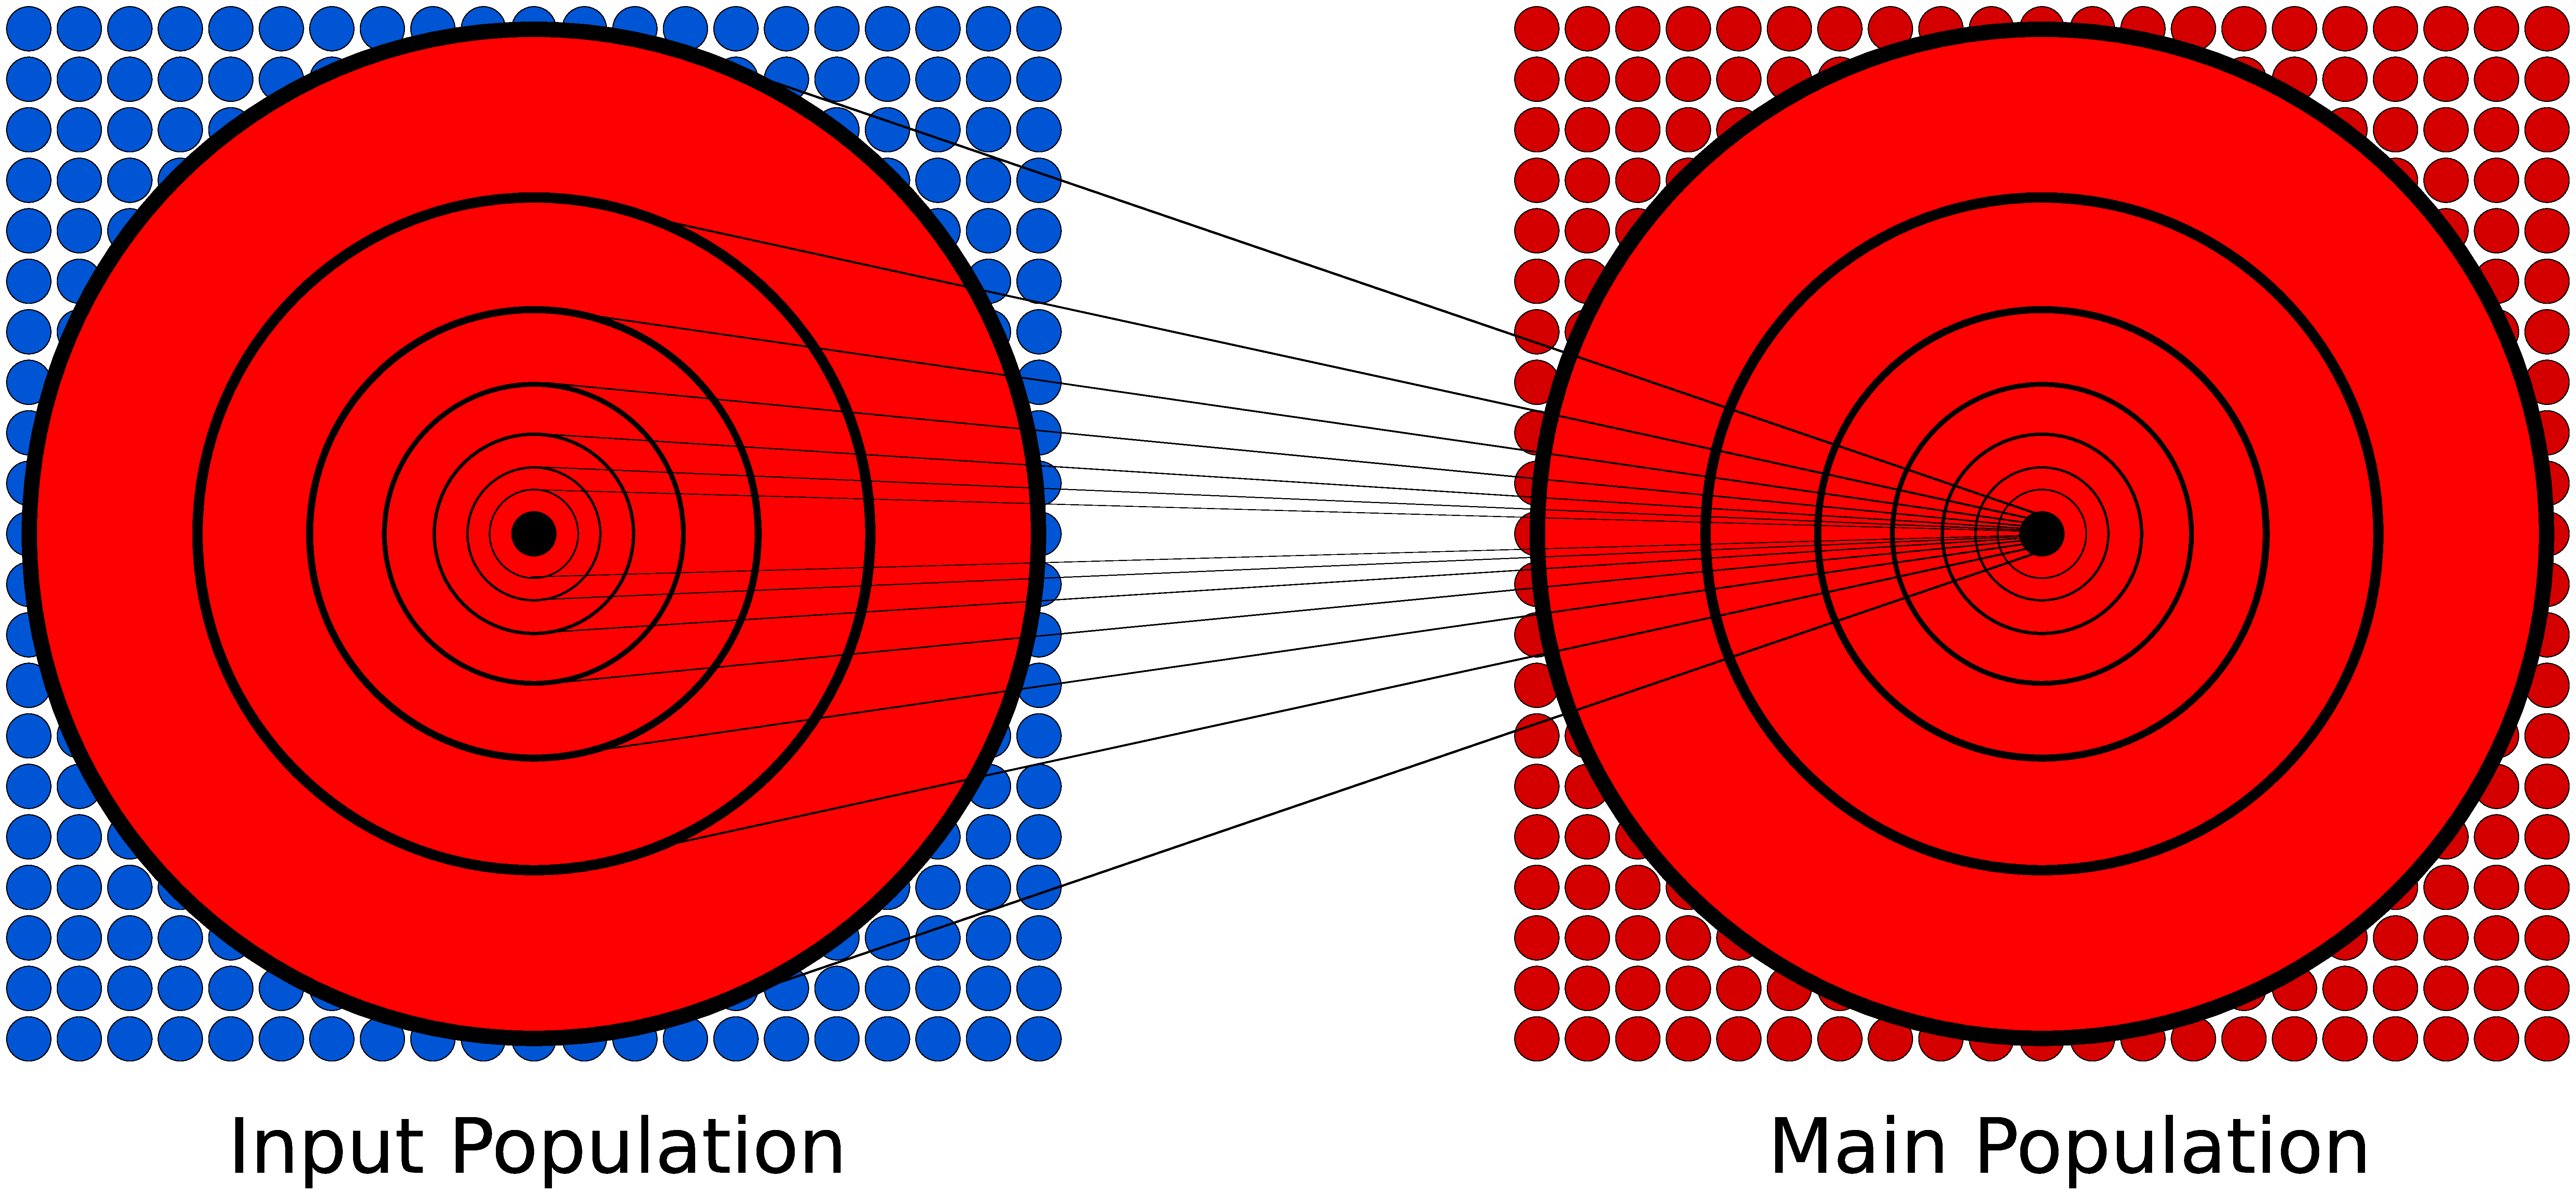
\epsfig{file=fieldsGaussians.eps, width=7cm}
  \caption{Neural fields for stability control (feedback with the
    plant not shown).}
\end{figure}


\section{Evolution of Neural Field Controllers}
\subsection{Evolutionary Algorithm Structure and Parameters}
For the evolution process it is used a simple evolutionary algorithm
as shown in the preliminaries, with random elimination of individuals
inversely proportional with their fitness.

The evolution parameters are the connection kernels between the input
layer and the processing layer, and the recurrent connections of the
processing layer with itself. The connection kernels are considered
isotropic and homogeneous along the field, so that they can be
described as symmetric one-dimensional arrays of values.

\subsection{Genotypic Representation and Evolution Operators}
Each connection kernel can be represented as an array of $N$ values
from $w(0)$ to $w(p)$ with homogeneous spacing, using their
symmetry. This way, for an equal boundary radius for all the kernels,
and a 2-layered architecture, there are $2N$ real values in the
genotype. As can be seen, the number of evolution parameters does not
have a direct relation with the simulation size of the neural fields
(the number of discrete points used), in contradistinction with
recurrent neural networks, where the number of parameters depends on
the number $n$ of neurons with a polynomial order
$O(n^2)$. Nonetheless, here is taken a more general approach and the
boundary radius is set equal to $n$, so that there are $O(n)$
parameters.

The evolution operations used in both steps are:
\begin{itemize}
\item Parametric mutation of input array: Gaussian modification of
  real codified array values, which varies the connection kernel
  between input layer and processing layer.
\item Parametric mutation of recurrence array: Gaussian modification
  of real codified array values, which varies the recurrent connection
  kernel of the processing layer.
\item Selection: Calculates population fitness, selects with elitism
  and culling (5\% of both) couples of parents for generating new
  offsprings, calculates the fitness function for both offsprings.
\end{itemize}

The mutation operators implemented apply the sum operator defined in
eq. ref{eq:eq-leb-opers} but there was not implemented a crossover
operator that used the scalar operator as it was not deemed necessary,
but can be easily implemented for another application if it is
considered useful.

\subsection{Fitness Function}
The fitness function is selected in such a way that the stability
controller mainly has the goal to reduce inclination. It was tuned
experimentally to attain a convergence velocity suitable for the
experiment. This has in mind a notion of sequential evolution of,
first, the capability to attain equilibrium, and later, the capability
to perturb the equilibrium controller in such a way that a planned
trajectory can be followed or a reference can be tracked. Here we are
interested only on the stability problem.

The fitness function for the stability controller is:

\begin{equation}
  F_1=100-\frac{100}{(\pi^4+2)T_{total}}\sum_t{\left(\theta(t) ^4+\frac{|x(t)|}{10}\right)}
\end{equation}

This fitness function aims to minimize the orientation error, but also
has as a minor second goal to minimize the total horizontal
displacement.


% \section{The RNN Controller Architecture}
% \label{sec:rnncontroller}
% % \subsection{RNN Controller Architecture for Comparison}
% The proposed architecture for the recurrent neural network controller
% has two expert recurrent networks, whose interaction will achieve
% positioning and equilibrium as well.

% There has been applied a preprocessing stage previous to the input
% neurons, so that the actual values are not used and instead the inputs
% are mapped to 3 fuzzy sets. In this way, the stability controller only
% has 3 inputs, while the positioning controller has 6, corresponding to
% the same 3 inputs previously described and another 3 due to the fuzzy
% mapping of the error signal. All neurons are interconnected and the
% first one of them is selected as output without loss of
% generality. The neural network topology for the first controller
% (stability) is shown in the figure \ref{fig:rnn-arch}.

% \begin{figure}[t]
%   \label{fig:rnn-arch}
%   \centering 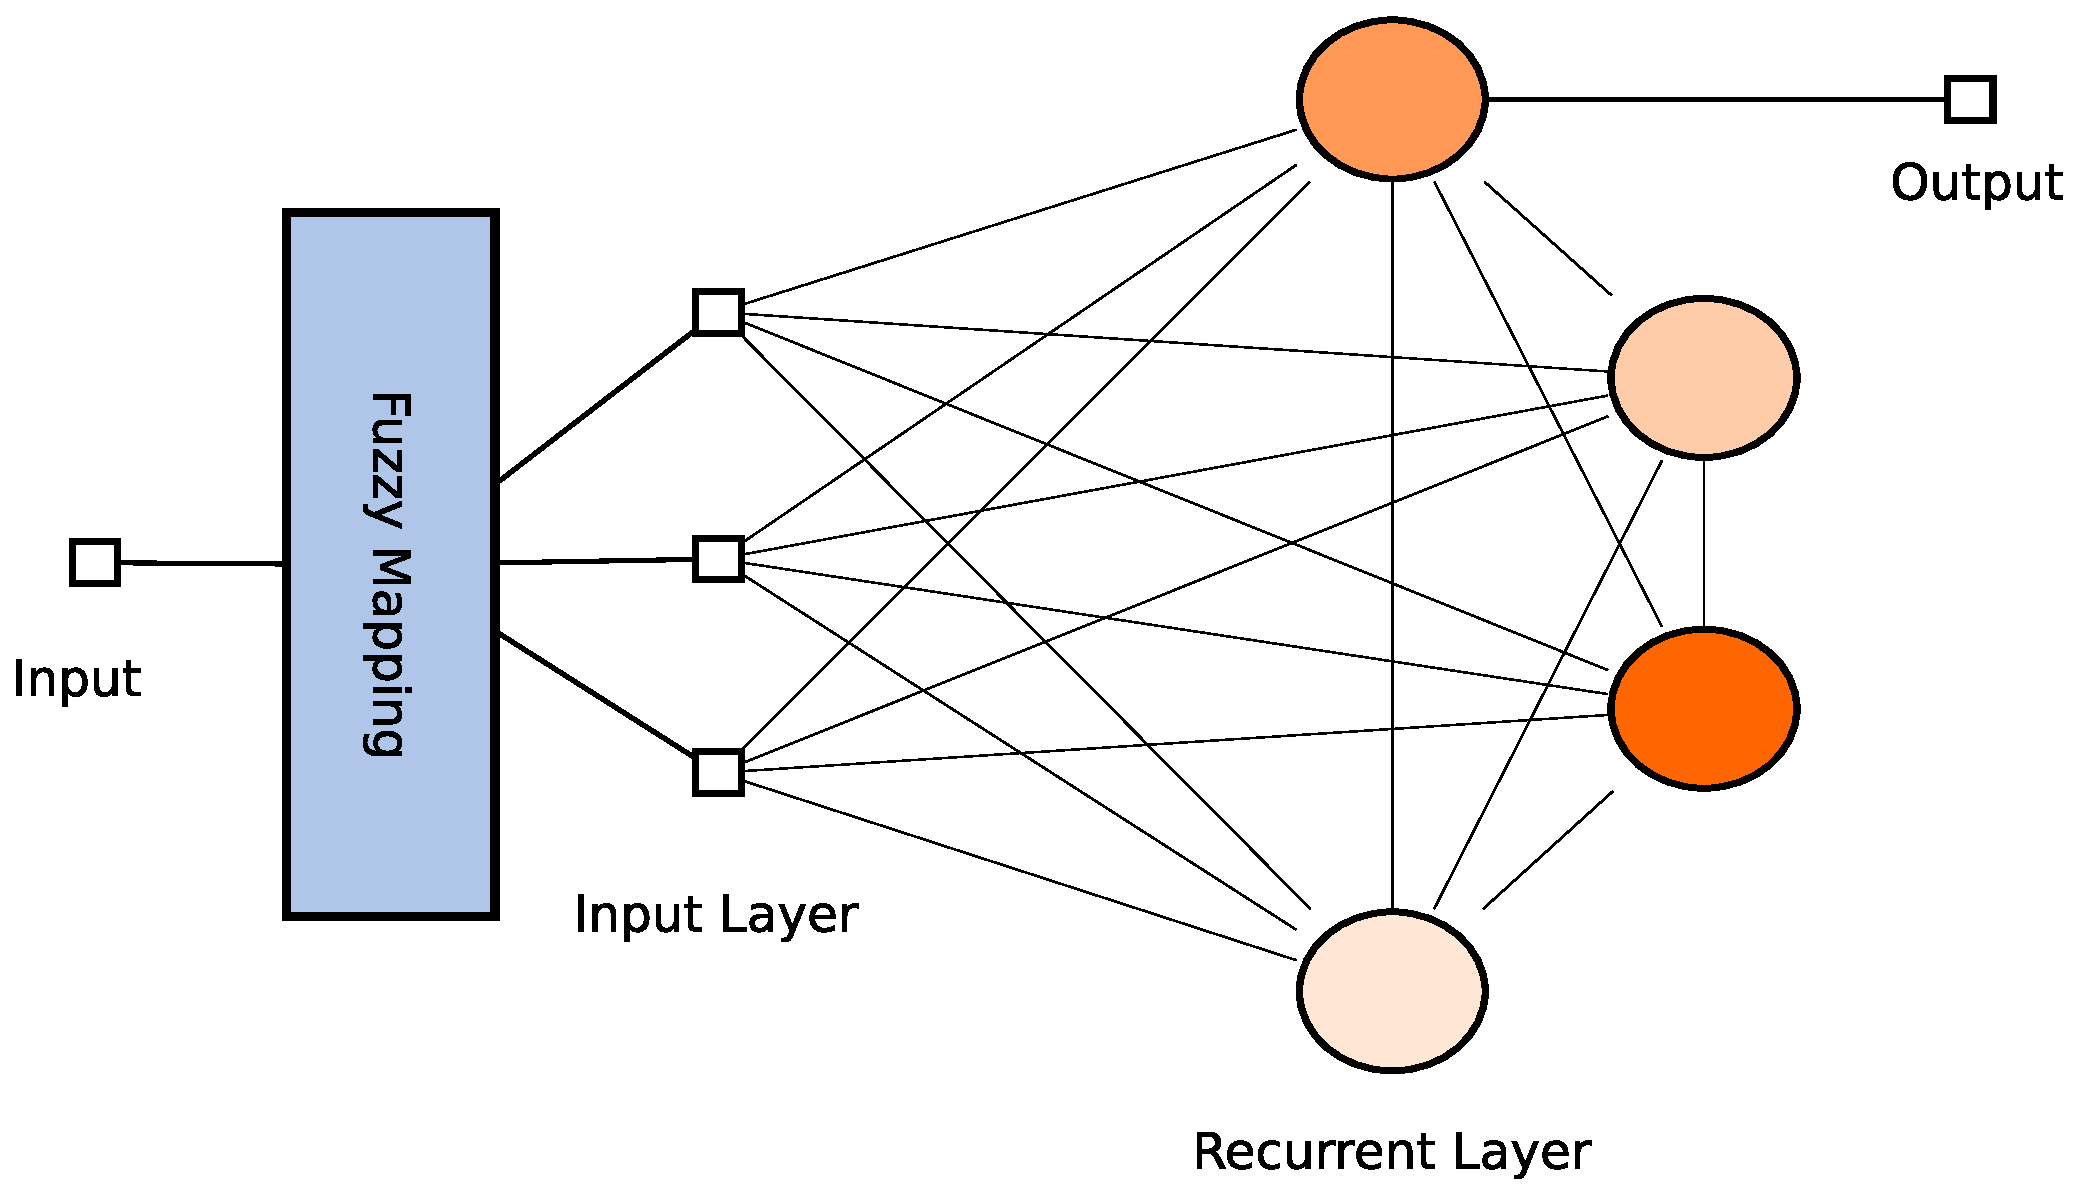
\epsfig{file=rnn.eps, width=7cm}
%   \caption{Neural net for stability control including fuzzy mapping}
%   \label{rnn}
% \end{figure}

% \subsection{Evolutionary Algorithm Structure for the RNN Controller}
% It is expected, based on the approach of artificial life to
% evolutionary robotics (Nolfi y Floreano), that the sequential and
% cooperative evolution of elements with biological similarity leads to
% an specialization in the process of stabilization and positioning
% (despite the antagonistic individual goals of each controller because
% of the interest of the positioning controller to maximize also the
% global performance).

% As said, the two steps are executed sequentially, taking the best
% individual of the first step to collaborate with the individual
% evolved in the second step.

% Aiming to obtain a fixed length representation and limit the problem
% dimensionality, it is used a model of order $Q$ totally connected. Any
% network with an order equal or lesser and with total or partial
% connections can be represented by the proposed model, by the addition
% of activating/deactivating elements for neurons and
% connections. Therefore, individual are codified as:

% \begin{itemize}
% \item A bit sequence representing a serialization of an activation
%   matrix $A_a$ of dimension $Q$-by-$Q$ which activates/deactivates a
%   recurrent connection.
% \item A sequence of real numbers representing a serialization of
%   matrices $W_a$ and $W_b$, of dimension $Q$-by-$Q$ and $Q$-by-$(m+1)$
%   respectively.
% \end{itemize}

% The $C$ matrix is not evolved because it is chosen arbitrarily only
% one output (the first neuron).

% The evolution operations used in both steps are:
% \begin{itemize}
% \item Parametric mutation of inputs: Gaussian modification of real
%   codified matrix weights, which varies connection weights of inputs.
% \item Parametric mutation of recurrences: Gaussian modification of
%   real codified matrix weights, which varies connection weights of
%   recurrences.
% \item Selection: Calculates population fitness, selects with elitism
%   and culling (5\% of both) couples of parents for generating new
%   offsprings, calculates the fitness function for both offsprings.
% \end{itemize}

% The fitness functions were selected in such a way that the stability
% controller only has the goal to reduce inclination. The fitness
% functions were tuned experimentally to attain a convergence velocity
% suitable for the experiment. This has in mind a notion of sequential
% evolution of, first, the capability to attain equilibrium, and later,
% the capability to perturb the equilibrium controller in such a way
% that a planned objective can be reached.

% The fitness function for the stability controller is:

% \begin{equation}
%   F_1(\theta )=100-\frac{100\theta ^4}{\theta _{max}^4 T_{total}}
% \end{equation}

% And for the positioning controller is:

% \begin{equation}
%   F_1(\theta ,e_x)=100-\frac{100(\theta ^4+e_x^4)}{(\theta _{max}^4+e_{x,max}^4) T_{total}}
% \end{equation}

% The fitness functions used are could be also applied to a evolution of
% the neural field controller.

\section{Experimental Results}
\subsection{Experimentation Details}
The sampling time used was $0.025$s (for neural networks, neural
fields, and visualization) and were performed $10$s tests.

The differential equation system was solved by a numerical method, 4th
Order Runge-Kutta. The iteration step selected was also $h=0.025s$ for
each test.

Here are shown the results for the proposed neural field architecture
without evolution and an appropriate selection of parameters (made
taking in account only the self-stability of the neural fields and the
time constants of the plant), and the evolution of a recurrent neural
network of a recurrent neural network controller. The initial angular
position was $\theta=\pi/6$ and the number of discrete positions used
in the simulation of the neural field was $21$. It was used the same
kernel and kernel parameters for the self connections of the
processing layer and the connections from the input layer to the
processing layer. The neural field time constant was taken with value
$\tau=1/10$s.

\subsection{Results}
The first experiment tests the physical model using the recurrent
neural network controller without evolution, to see the natural
dynamics of the system when the controller is configured arbitrarily
(in such a way that can be perceived the need of the evolutionary
algorithm for the recurrent neural network controller). Results are
shown in the figure \ref{inestabilidad}. As can be seen, it is an
unstable system in the origin. Red dots represent the pendulum
position referenced to universal coordinates, and blue dots represent
the base (car) position.


\begin{figure}[t]
  \centering 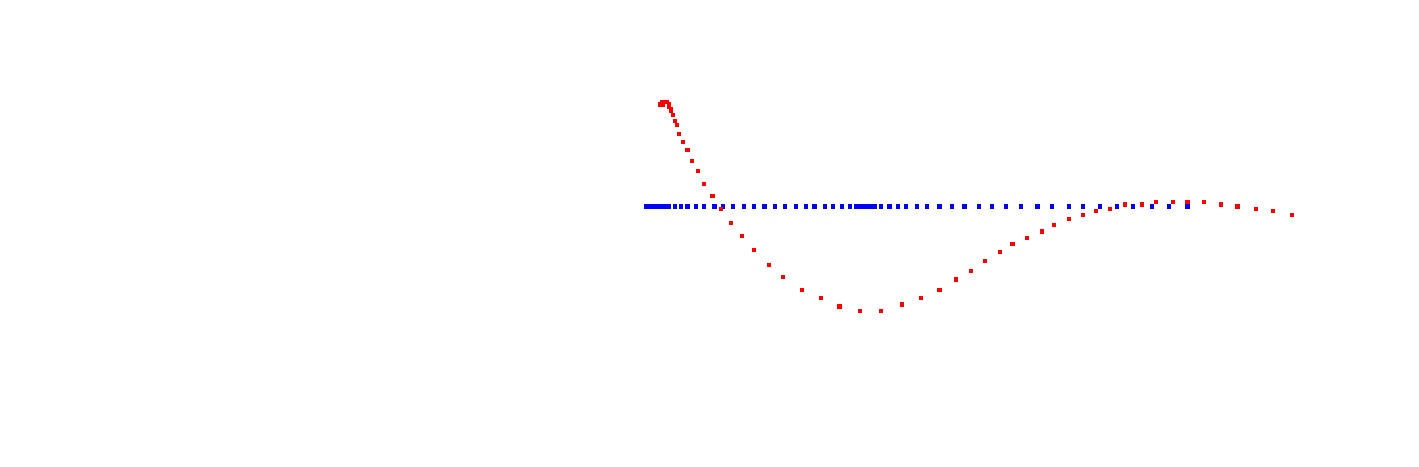
\epsfig{file=inestabilidadG.eps, width=7cm}
  \\
  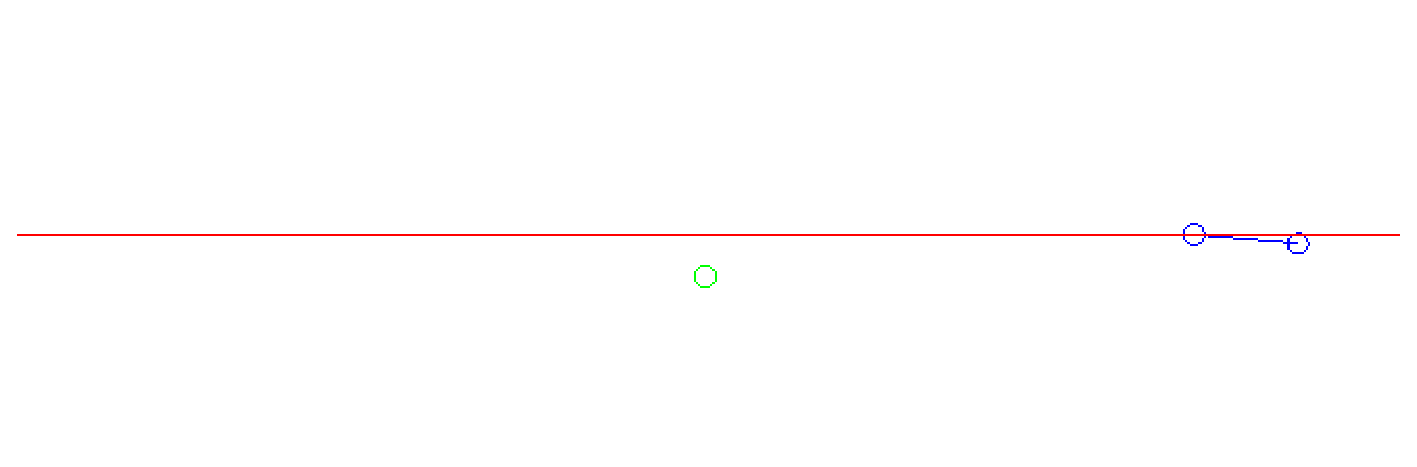
\epsfig{file=inestabilidadC.eps, width=7cm}
  \caption{System dynamics with an untrained RNN controller. The first
    figure shows the pendulum trace and the second the pendulum at a
    given time.}
  \label{inestabilidad}
\end{figure}

After the parameterization made by the evolutionary algorithm for the
RNN controller, it is shown the behavior of the controller in the
figure \ref{rnnSimulation}. The evolution was performed with a
population of 100 individuals and 500 iterations.

\begin{figure}[t]
  \centering 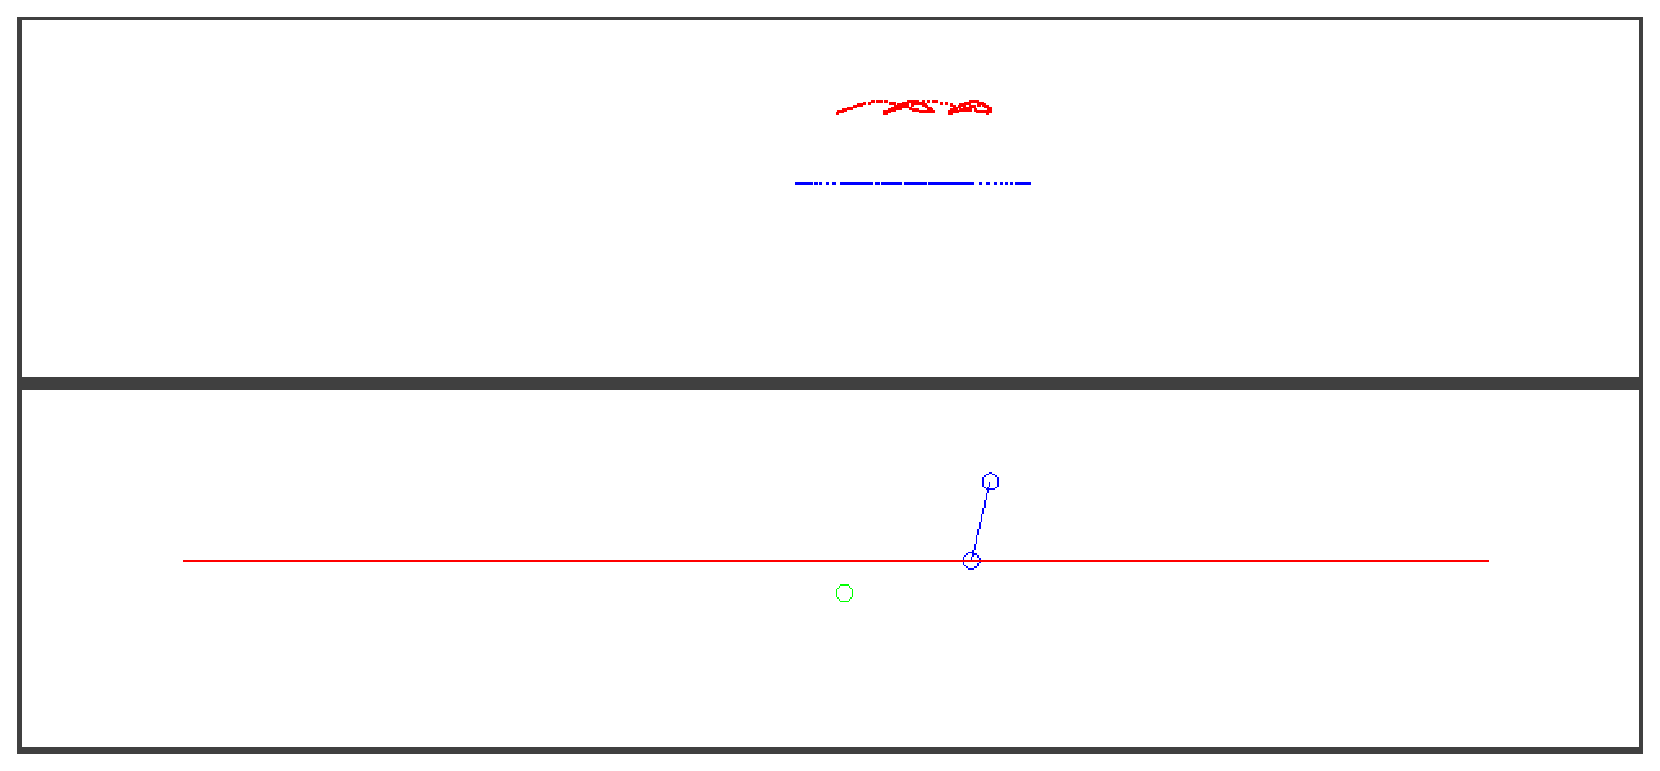
\epsfig{file=rnnSimulation.eps, width=7cm}
  \caption{System dynamics with a RNN controller trained. The first
    figure shows the pendulum trace and the second the pendulum at
    $t=3.5$s.}
  \label{rnnSimulation}
\end{figure}

On the other hand, the neural field is able to control the stability
without evolution with a performance similar (or even better) than the
presented by the evolved RNN controller. The simulation is shown in
the figure \ref{fieldSimulation}, including the neural field values at
a given point of time. Different $k_{\omega}$ values affected the
system response but kept the system stable.


\begin{figure}[p]
  \centering 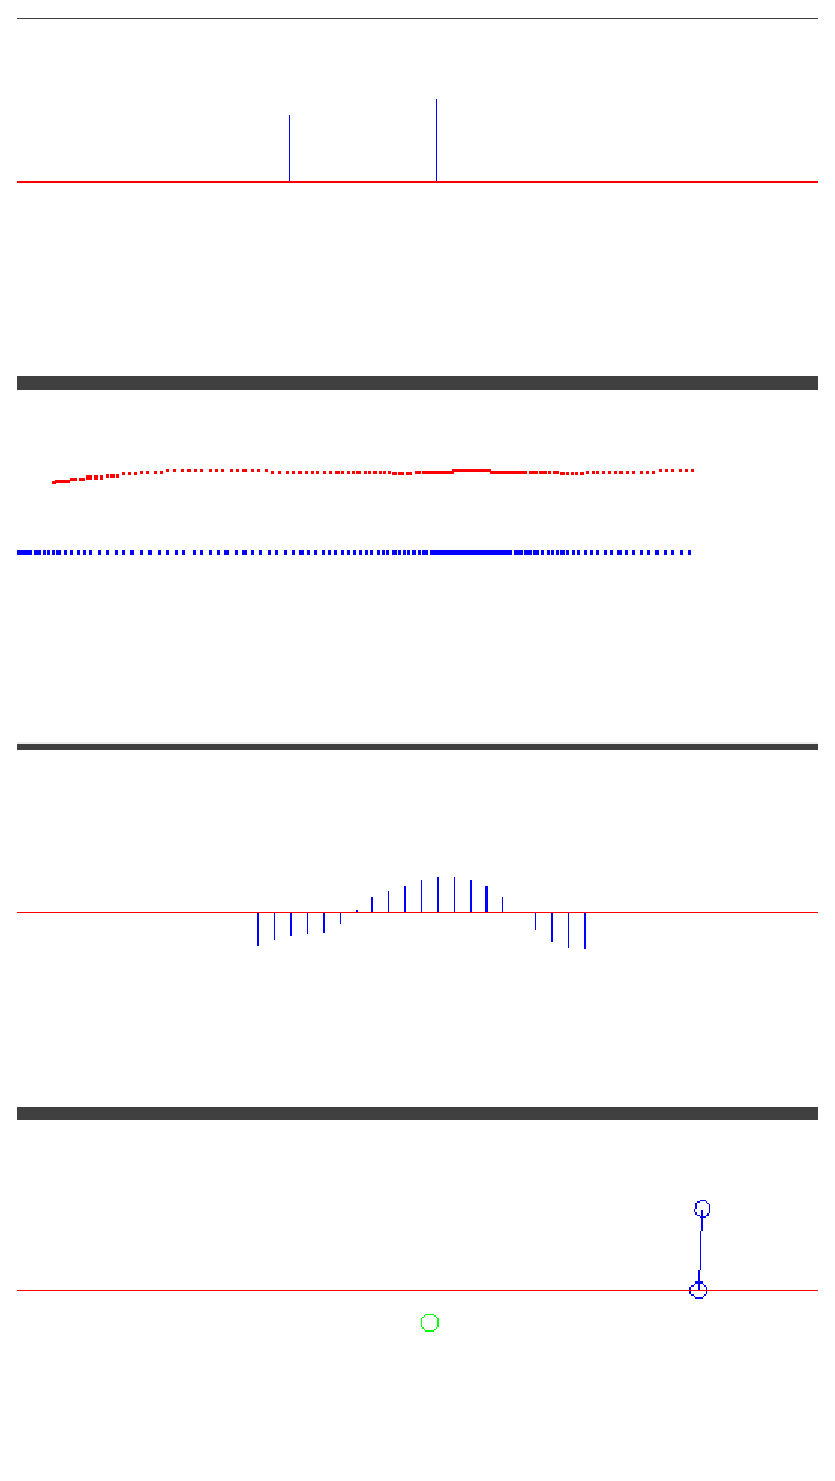
\epsfig{file=neuralfield-panel-1.eps, width=7cm}
  \caption{System dynamics with a non-trained Neural Field
    Controller. In order: the input layer at time $t=3.5$, the
    pendulum trace, the processing layer at time $t$, and the pendulum
    at time $t$.}
  \label{fieldSimulation}
\end{figure}

A detailed evolution of the neural field controller can be seen in the
figure \ref{fig:nf-controller}.

\begin{figure}[t]
  \centering \epsfig{file=inputPopulation.eps, width=7cm}
  \epsfig{file=fieldPopulation.eps, width=7cm}
  \caption{Neural Field simulation between $t=0$s and $t=10$s with
    steps $h=1/40$s and positions between $x_{min}=-10$ and
    $x_{max}=10$. First figure is the input layer activation, with
    $\theta$ input with value $1$ and $\dot{\theta}$ with value
    $k_{\omega}=0.8$. The second figure is the processing layer
    activation.}
  \label{fig:nf-controller}
\end{figure}

And a detailed evolution of the pendulum with the neural field
controller can be seen in the figure \ref{fig:nf-pendulum}.

\begin{figure}[t]
  \centering \epsfig{file=pendulum.eps, width=7cm}
  \caption{Pendulum simulation with neural field controller between
    $t=0$s and $t=10$. Each state is coded with a position (so that
    the pendulum can be simulated as a field on its own) this way:
    $x$:0, $\theta$:1, $\dot{x}$:2, $\dot{\theta}$:3. It can be seen
    the little variation in the angular position ($\theta$). The
    discontinuity in $x$ is present because position wraps in the
    simulation so that $x=5$ is equivalent to $x=-5$.}
  \label{fig:nf-pendulum}
\end{figure}



\section{Conclusions}
While the recurrent neural network controller is expressive enough to
solve the problem at hand, the number of parameters to configure (or
in this case to evolve) is of a quadratic order in relation to the
number of nodes (or neurons). This was not a particular problem for
the evolutionary algorithm used, but limits its potential
scalability. Furthermore, while it is expressive enough, does not show
a particular suitability (needs explicit and specific
parameterization) to the dynamic stability problem of the inverted
pendulum and there are no reasons to expect something different for a
more complex biped model.

On the other hand, the neural field controller is a bit more complex
(in its implementation) and its simulation more costly, but has some
notable advantages. The first one is its ability to self-compensate
or, equivalently, the stability of its natural dynamics, which is
attained after the setup of few parameters. The second one is its
suitability to the problem at hand, being able to solve it with a good
performance for low perturbations. Although there was a need for
parameter configuration, evolution was not required because the small
number of parameters to setup: basically three parameters of the
kernel function and the resting potential of the field equation - a
number of parameters of constant order in relation to the number of
nodes (discrete potentials on the neural field).

Remarkably, the non-evolved neural field controller performs as good
or better than the evolved recurrent neural network
controller. Furthermore, the neural field has a spatial representation
which allows interpretation of field potentials (as shown in
fig. \ref{fig:nf-controller}). The interpretation or understanding of
recurrent neural networks is quite difficult and even more with
increasing states involved. This makes the neural field controller not
as black-box as the RNN controller.

More complex control problems seem to require an strategy of
parameterization of the neural field controller. This way, it is left
for future work the task of neural field evolution as it was briefly
presented in section \label{sec:properties}.

\bibliographystyle{abbrv} \bibliography{bibanot}

\end{document}
